\section{Jednadžba gibanja modela pri sinusnoj pobudi}
Dijagram sila za sustav s prigušenjem na koji djeluje sila pobude $p(t)$ prikazan je
na slijedećoj slici:

\begin{figure}[H]
    \begin{subfigure}[b][][l]{0.5\textwidth}
        \begin{tikzpicture}
%povecaj strelice
\tikzset{myptr/.style={decoration={markings,mark=at position 1 with %
    {\arrow[scale=2,>=stealth]{>}}},postaction={decorate}}}

	%podloga
%	\draw[white, pattern=north east lines, pattern color=black] (0, 0)
%	rectangle (-0.5, 2.2);
%	\draw[thick] (0,0) -- (0, 2.2);

%	\draw[white, pattern=north east lines, pattern color=black] (0, 0) 
%	rectangle (5, -0.5);
%	\draw[thick] (0,0) -- (5,0);
	
%	\draw[white, pattern=north east lines, pattern color=black] (0, 0)
%	rectangle (-0.5, -0.5);

	%uteg
	\filldraw[fill=black] (1.5, 2) rectangle (3.5, 0.25);

	%kotaci
	\filldraw[fill=black] (2, 0.125) circle (0.125);
	\filldraw[fill=black] (3, 0.125) circle (0.125);

	%sile
	\draw[myptr] (1.5, 1.5625) -- (0.25, 1.5625) 
		node[pos=1, above]{\textbf{\large{$F_s$}}};
	\draw[myptr] (1.5, 0.6875) -- (0.25, 0.6875)
		node[pos=1, below]{\textbf{\large{$F_d$}}};
	\draw[myptr] (3, 1.125) -- ( 5.25, 1.125) 
		node[pos=1, above]{\textbf{\large{$p(t)$}}};

\end{tikzpicture}

        \caption{}
        \label{fig:sile-priguseni-ekvivalentni-sustav-sdf}
    \end{subfigure}
    \hfill
    \begin{subfigure}[b][][r]{0.5\textwidth}
        \begin{tikzpicture}
%povecaj strelice
\tikzset{myptr/.style={decoration={markings,mark=at position 1 with %
    {\arrow[scale=2,>=stealth]{>}}},postaction={decorate}}}

	%podloga
%	\draw[white, pattern=north east lines, pattern color=black] (0, 0)
%	rectangle (-0.5, 2.2);
%	\draw[thick] (0,0) -- (0, 2.2);

%	\draw[white, pattern=north east lines, pattern color=black] (0, 0) 
%	rectangle (5, -0.5);
%	\draw[thick] (0,0) -- (5,0);
	
%	\draw[white, pattern=north east lines, pattern color=black] (0, 0)
%	rectangle (-0.5, -0.5);

	%uteg
	\filldraw[fill=gray] (1.5, 2) rectangle (3.5, 0.25);

	%kotaci
	\filldraw[fill=gray] (2, 0.125) circle (0.125);
	\filldraw[fill=gray] (3, 0.125) circle (0.125);

	%sile
	\draw[myptr] (1.5, 1) -- (0.25, 1) 
		node[pos=1, above]{\textbf{\large{$F_s$}}};
	\draw[myptr] (3.5, 1) -- ( 4.75, 1) 
		node[pos=1, above]{\textbf{\large{$p(t)$}}};

\end{tikzpicture}

        \caption{}
        \label{fig:sile-nepriguseni-ekvivalentni-sustav-sdf}
    \end{subfigure}
    \caption{Dijagram sila;
        (\subref{fig:sile-priguseni-ekvivalentni-sustav-sdf})
            prigušenog sustava; 
    (\subref{fig:sile-nepriguseni-ekvivalentni-sustav-sdf})
            neprigušenog sustava}
    \label{fig:dijagrami_sila}
\end{figure}


Prema drugom Newtonovom aksiomu vrijedi:
\begin{align}
    \Sigma F = ma = m\ddot{u}\notag\\
        p(t) - F_S - F_D = m\ddot{u} \notag\\
        m\ddot{u} + F_S + F_D = p(t) \label{eq:newton}
\end{align}

Gdje je:\\
\begin{table}[H]
\begin{tabular}{c l}
	$F_S$ & unutarnja sila \\
	$F_D$ & sila prigušenja \\
	$m$   & masa \\
        $a,\ddot{u}$   & ubrzanje\\
\end{tabular}
\end{table}

Unutarnju silu možemo zapisati kao:
\begin{equation}
	F_S = k \cdot u \label{eq:hooke}
\end{equation}

A silu prigušenja kao:
\begin{equation}
	F_D = c \cdot v = c \cdot \dot{u} \label{eq:prigusenje}
\end{equation}

Gdje je:\\
\begin{table}[H]
\begin{tabular}{c l}
	$k$ & krutost \\
	$c$ & koeficijent viskoznog prigušenja \\
	$u$ & pomak \\
	$\dot{u},v$ & brzina \\
\end{tabular}
\end{table}

Uvrštavanjem \eqref{eq:hooke} i \eqref{eq:prigusenje} u \eqref{eq:newton} dobijemo:
\begin{equation}
	m\ddot{u} + c\dot{u} + ku = p(t) \label{eq:jednadzba_opcenita_pobuda}
\end{equation}

Sila pobude $p(t)$ je sinusna sila $p_0sin(\omega t)$, pri čemu je $p_0$ amplituda, a
$\omega$ frekvencija, stoga jednadžba pod \eqref{eq:jednadzba_opcenita_pobuda}
postaje:
\begin{equation}
	m\ddot{u} + c\dot{u} + ku = p_0sin(\omega t)
\label{eq:jednadzba_sinusna_pobuda}
\end{equation} 


Jednadžba pod \eqref{eq:jednadzba_sinusna_pobuda} jest nehomogena linearna
diferencijalna jednadžba drugog reda, a riještiti ćemo ju primjenom Laplaceove
transformacije\footnote{Iako postupkom dugotrajnija (u ovom
slučaju), metoda Laplaceove transformacije nam pruža jedinstven uvid u međudjelovanje sustava
i pobude.}.
\par

Transformiranjem jednadžbe \eqref{eq:jednadzba_sinusna_pobuda} dobijemo 
slijedeću algebarsku jednadžbu u frekvencijskoj domeni:
\begin{equation}\label{eq:transformat_diferencijalna}
        m(s^2U(s)-su(0)-\dot{u}(0))+
	c(sU(s)-u(0))+
	kU(s) = 
        P(s)
\end{equation}
Gdje je $P(s)$ transformat funkcije $p(t)=p_0\sin(\omega t)$.
Sređivanjem \eqref{eq:transformat_diferencijalna} dobijemo: 
\begin{equation}\label{eq:transformat_diferencijalna_sredjeno}
    U(s)\left(ms^2+cs+k\right)-msu(0)-m\dot{u}-cu(0) = P(s)
\end{equation}

Jednadžbu \eqref{eq:transformat_diferencijalna_sredjeno} možemo rastaviti na više logičnih
cijelina:
\begin{alignat}{2}
    &\text{Dinamička krutost} & Z(s)&=ms^2+cs+k\label{eq:din_krutost}\\
    &\text{Prijenosna funkcija sustava}\quad & H(s)&=\frac{1}{Z(s)}=\frac{1}{ms^2+cs+k}\label{eq:prijenosna}\\
    &\text{Pobuda početnim uvjetima}\quad & W(s)&=(ms+c)u(0)+m\dot{u}\label{eq:pobuda_pocetni}\\
    &\text{Pobuda sinusnom silom} & P(s)&=p_0\frac{\omega}{s^2+\omega^2}\label{eq:pobuda_sinusna}
\end{alignat}

Uvrštavanjem \eqref{eq:prijenosna},\eqref{eq:pobuda_pocetnim_uvjetima} u 
\eqref{eq:transformat_diferencijalna_sredjeno} dobijemo:
\begin{equation*}
	\frac{U(s)}{H(s)}=W(s)+P(s)
\end{equation*}

Množenjem prijenosnom funkcijom sustava ($H(s)$) dobijemo:
\begin{equation}
	U(s)=\underbrace{H(s)W(s)}_{\substack{\text{konvolucija u}\\\text{vremenskoj
	domeni}}}
	+ 
	\underbrace{H(s)P(s)}_{\substack{\text{konvolucija u}\\\text{vremenskoj domeni}}}
\end{equation}

Pri čemu je:
\begin{table}[H]
\begin{tabular}{c l}
	$H(s)\cdot W(s)$ & odziv na pobudu početnim uvjetima u frekvencijskoj domeni\\
	$H(s)\cdot P(s)$ & odziv na pobudu sinusnom silom u frekvencijskoj domeni\\
\end{tabular}
\end{table}

\newpage
Da bi bilo lakše naći inverze odziva u frekvencijskoj domeni potrebno je funkciju  
$H(s)$ prikazati u tabličnom obliku\footnote{postupak svođenja prijenosne funkcije
sustava na tablični oblik prikazan je u slijedećem pogavlju}.

\begin{equation}\label{eq:pfs_tablicni_oblik}
    H(s) = \frac{\omega_n^2}{\omega_D}
           \frac{1}{k}
           \frac{\omega_D}{(s+\sigma)^2+\omega_D^2}
\end{equation}

Gdje je:\\
\begin{table}[H]
    \begin{tabular}{r l}
        $\sigma=\zeta\omega_n$ & stupanj prigušenja\\
        $\omega_D=\omega_n\sqrt{1-\zeta^2}$ & vlastita frekvencija prigušenog titranja\\
        $\omega_n=\sqrt{k/m}$ & prirodna frekvencija oscilatora\\
        $\zeta=c/c_{kr}$ & koeficijent relativnog prigušenja\\
        $c_{kr}=2m\omega_n$ & kritično prigušenje
    \end{tabular}
\end{table}

Pobuda početnim uvjetima zadana je preko jednadžbe:
\begin{equation}
    \begin{split}
        H(s)W(s)=\frac{u_0}{\omega_D}&\left(
        \frac{s+\sigma}{(s+\sigma)^2+\omega_D^2} +
	\sigma\frac{\omega_D}{(s+\sigma)^2+\omega_D^2}\right)\\
        &+ \frac{\dot{u}(0)}{\omega_D}\frac{\omega_D}{(s+\sigma)^2+\omega_D}
    \end{split}
\end{equation}

Odziv u vremenskoj domeni se određuje pronalaskom inversa $\ltr$ transformacije
funkcije odziva u frekvencijskoj domeni.
\begin{equation}
	u(t)=\ltr^{-1}\{U(s)\}=\ltr^{-1}\{W(s)H(s)\}+\frac{p_0}{k}\ltr^{-1}\{H(s)P(s)\}
	\label{eq:inverz_prvi_korak}
\end{equation}

Funkcija $H(s)W(s)$ svedena je na tablični oblik stoga je moguće izravno naći inverz
Laplaceove transformacije koji glasi:
\begin{equation}
	\ltr^{-1}\{H(s)W(s)\} = e^{-\sigma t}\left[
		u(0)cos(\omega_Dt)+\left(
			\sigma\frac{u(0)}{\omega_D}+\frac{\dot{u}(0)}{\omega_D}
			\right)sin(\omega_Dt)\right] \label{eq:pobuda_pocetnim_uvjetima}
\end{equation}

Funkciju $H(s)P(s)$ nije moguće svesti na tablični oblik, pa je potrebno odrediti
konvoluciju funkcija $h(t)$ i $p(t)$. Funkcija funkcija $H(s)$ odgovara funkciji 
$h(t)$ u vremenskoj domeni, a funkcija $P(s)$ funkciji $p(t)$, stoga:
\begin{align}
        h(t)&=\ltr^{-1}\{H(s)\}=\frac{1}{k}\frac{\omega_n^2}{\omega}e^{-\sigma t}sin(\omega_Dt)\label{eq:pfs_vremenska_domena}\\
	p(t)&=\ltr^{-1}\{P(s)\}=p_0\sin(\omega t) \label{eq:pobuda_vremenska_domena}
\end{align}

Konvoluciju funkcija određujemo preko konvolucijskog integrala:
\begin{align}\label{eq:konvolucijski_integral}
	(h*p)(t)&=\int_0^th(\tau)p(t-\tau)d\tau \notag\\
		&=\frac{p_0}{k}\frac{\omega_n^2}{\omega}
		\int_0^te^{-\sigma\tau}sin(\tau)sin(t-\tau)d\tau
\end{align}

Ukupni odziv je suma odziva na pobudu početnim uvjetima i odziva na pobudu
harmonijskom silom odnosno:
\begin{equation}
    \begin{split}
    u(t)&=\underbrace{e^{-\sigma t}\left[
		u(0)cos(\omega_Dt)+\left(
                        \sigma\frac{u(0)}{\omega_D}+\frac{\dot{u}(0)}{\omega_D}
                        \right)sin(\omega_Dt) \right]}_{\text{\textbf{pobuda
                    početnim uvjetima (prolazni dio odziva)}}}\\
                    &+\underbrace{
                        \frac{p_0}{k}
                        \frac{\omega_n^2}{\omega_D}
                        \int_0^te^{-\sigma\tau}\sin(\tau)\sin(t-\tau)d\tau
                    }_{\text{\textbf{pobuda sinusnom silom}}}
    \end{split}
    \label{eq:inverz_drugi_korak}
\end{equation}

Postupak određivanja i sređivanja rješenja konvolucijskog integrala iz
\eqref{eq:konvolucijski_integral} je dugotrajan pa je u nastavku prikazano samo konačno 
rješenje.
\begin{equation}
	\begin{split}
	(p*h)(t)&=\underbrace{
			Csin(\omega t)+Dcos(\omega t)
		}_{\text{\textbf{prisilni dio odziva}}}\\
		&-
		\underbrace{
			e^{-\sigma t}
				\left(
				Dcos(\omega_D t) +
					\left(
						\frac{D\sigma}{\omega_D}+\frac{C\omega}{\omega_D}
					\right)
				sin(\omega_Dt)
				\right)
		}_{\text{\textbf{prolazni dio odziva}}}
	\end{split}
    \label{eq:konvolucijski_integral_rjesenje}
\end{equation}

Gdje je:
\begin{align}
    C &= \frac{p_0}{k}\frac{1-(\omega/\omega_n)^2}
            {[1-(\omega/\omega_n)^2]^2+[2\zeta\omega/\omega_n]^2}\label{eq:koef_C}\\
    D &= \frac{p_0}{k}\frac{-2\zeta\omega/\omega_n}
            {[1-(\omega/\omega_n)^2]^2+[2\zeta\omega/\omega_n]^2]}\label{eq:koef_D}
\end{align}

Iz \eqref{eq:konvolucijski_integral_rjesenje} i \eqref{eq:inverz_drugi_korak} možemo
zaključiti da će se prolazni dio odziva pojaviti i u slučaju homogenih i u slučaju
nehomogenih početnih uvjeta (prisutan i kod pobude početnim uvjetima i kod pobude
silom), a ovisi o karakteristikama sustava,
te se smanjuje eksponencijalno u ovisnosti o vremenu. Nakon
što prolazni dio odziva isčezne preostaje samo prisilni dio odziva, a pojavljuje se
neovisno o početnim uvjetima. Karakteristike prisilnog dijela odziva ponajviše ovise
o frekvenciji i amplitudi pobude, a zatim i o karakteristikama sustava (o prigušenju
te prirodnoj frekvenciji sustava). Karakteristike prisilnog dijela odziva detaljnije će se
razmatrati u slijedećim poglavljima.
\newpage

Uvrštavanjem \eqref{eq:konvolucijski_integral_rjesenje} u
\eqref{eq:inverz_drugi_korak}, te sređivanjem dobijemo ukupno rješenje
diferencijalne jednadžbe \eqref{eq:jednadzba_sinusna_pobuda} koje glasi:
\begin{equation}\label{eq:inverz_treci_korak}
	u(t)=\underbrace{
		e^{-\sigma t}(Acos(\omega_D t)+Bsin(\omega_Dt)
		}_{\text{\textbf{prolazni dio odziva}}}
		+
	     \underbrace{
		Csin(\omega t) + Dcos(\omega t)
		     }_{\text{\textbf{prisilni dio odziva}}}
\end{equation}

Gdje je:
\begin{align}
    A &= u(0)-D\label{eq:koef_A}\\
    B &= \frac{u(0)\sigma}{\omega_D}+
         \frac{\dot{u}(0)}{\omega_D}-
         \frac{D\sigma}{\omega_D}-
         \frac{C\omega}{\omega_D}\label{eq:koef_B}
\end{align}

Graf odziva prigušenog sustava s jednim stupnjem slobode za homogene početne
uvjete $u(0)=0$ i $\dot{u}(0)=0$ prikazan je na slijedećoj slici.
\begin{figure}[H]
    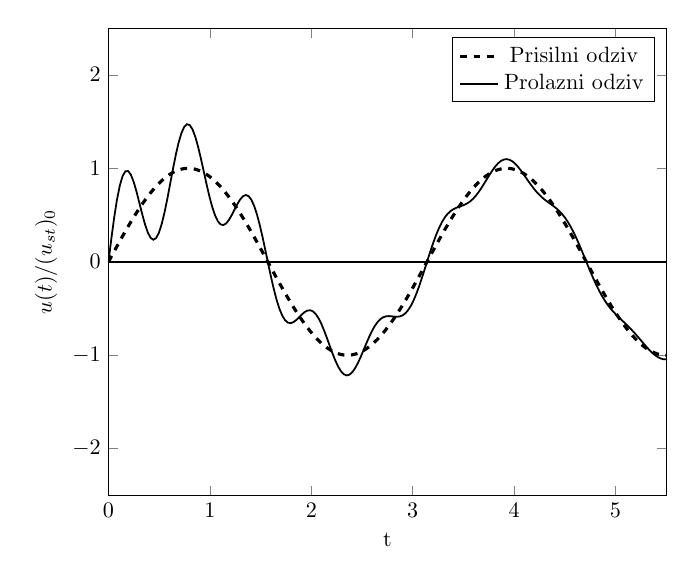
\begin{tikzpicture}[scale=0.8]
    \begin{axis} [
        height=9cm,
%        axis lines = center,
        xlabel=t,ylabel=$u(t)/(u_{st})_0$,
        ylabel near ticks, ylabel style={anchor=south},
        xmin = 0, xmax = 5.5,
        ymin = -2.5, ymax = 2.5,
        xtick = {0, 1, 2, 3, 4, 5},
        ytick = {-2,-1, 0, 1, 2},
     ]
        \addplot [
            domain=0:5.5,
            samples=200,
            color=black,
            dashed,line width=0.5mm,
        ] {sin(2*deg(x))};
        \addlegendentry{Prisilni odziv}
        \addplot [
            domain=0:5.5,
            samples=200,
            color=black,
            thick,
        ] {sin(2*deg(x))+0.7*exp(-0.05*10*x)*sin(10*deg(x))};
        \addlegendentry{Prolazni odziv}
    \draw[thick] (0,0)--(5.5,0);
    \end{axis}
\end{tikzpicture}

    \label{fig:odziv-priguseno}
    \caption{Odziv prigušenog sustava na pobudu sinusnom silom za
    $\omega/\omega_n=0.2$ i $\zeta=0.05$}
\end{figure}
\newpage

Neprigušeni sustav možemo shvatiti kao poseban slučaj prigušenog sustava za slučaj
$c=0$ odnosno $\zeta=0$, pa diferencijalna jednadžba sustava postaje:
\begin{equation}\label{eq:jednadzba_gibanja_nepriguseni_nesredjeno}
	m\ddot{u}+ku=p(t)
\end{equation}

Rješenje jednadžbe gibanja možemo odrediti iz \eqref{eq:inverz_treci_korak}
određivanjem koeficijenata $A$, $B$, $C$ i $D$ za $\zeta = 0$.
\begin{align}
    A &= u(0) \label{eq:np_koef_A}\\
    B &= \frac{\dot{u}(0)}{\omega_n}-\frac{\omega/\omega_n}{1-(\omega/\omega_n)^2}\label{eq:np_koef_B}\\
    C &= \frac{p_0}{k}\frac{1}{1-(\omega/\omega_n)^2}\label{eq:np_koef_C}\\
    D &= 0\label{eq:np_koef_D}\\
    \sigma &= \omega_n\zeta=\omega_n\cdot 0=0\label{eq:np_sigma}\\
    \omega_D &= \omega_n\sqrt{1-\zeta^2}=\omega_n\sqrt{1-0}=\omega_n\label{eq:np_omega_D}
\end{align}

Uvrštavanjem \eqref{eq:np_koef_A}, \eqref{eq:np_koef_B}, \eqref{eq:np_koef_C},
\eqref{eq:np_koef_D}, \eqref{eq:np_sigma} i \eqref{eq:np_omega_D} u  \eqref{eq:inverz_treci_korak}
dobijemo rješenje diferencijalne jednadžbe pod
\eqref{eq:jednadzba_gibanja_nepriguseni_nesredjeno} 
koje glasi:
\begin{equation}
	u(t)=\underbrace{
            u(0)cos(\omega_n t)
	\left[
		\frac{\dot{u}(0)}{\omega_n}-\frac{\omega/\omega_n}{1-(\omega/\omega_n)^2}
        \right]sin(\omega_n t)\\
	}_{\text{\textbf{prolazni dio odziva}}}
        +
	\underbrace{
		\frac{1}{1-(\omega/\omega_n)^2} sin(\omega t)
	}_{\text{\textbf{prisilni dio odziva}}}
\end{equation}

\begin{figure}[H]
    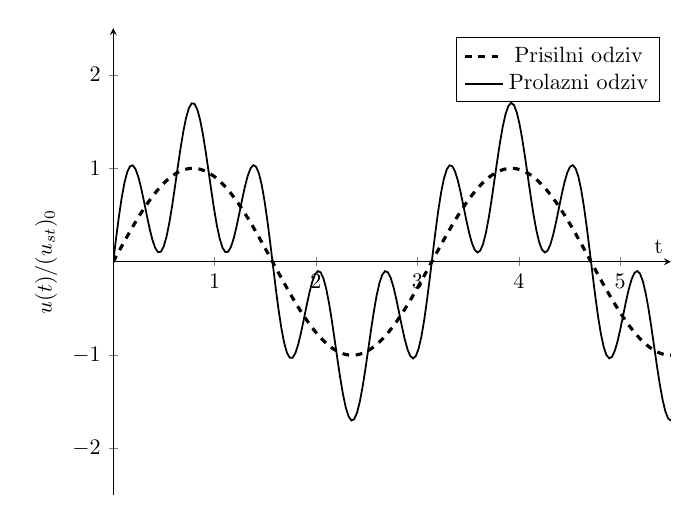
\begin{tikzpicture}[scale=0.8]
    \begin{axis} [
        height=9cm,
        axis lines = center,
        xlabel=t,ylabel=$u(t)/(u_{st})_0$,
        ylabel near ticks, ylabel style={anchor=south},
        xmin = 0, xmax = 5.5,
        ymin = -2.5, ymax = 2.5,
        xtick = {0, 1, 2, 3, 4, 5},
        ytick = {-2,-1, 0, 1, 2},
     ]
        \addplot [
            domain=0:5.5,
            samples=200,
            color=black,
            dashed,line width=0.5mm,
        ] {sin(2*deg(x))};
        \addlegendentry{Prisilni odziv}
        \addplot [
            domain=0:5.5,
            samples=200,
            color=black,
            thick,
        ] {sin(2*deg(x))+0.7*sin(10*deg(x))};
        \addlegendentry{Prolazni odziv}

    \end{axis}
\end{tikzpicture}

    \label{fig:odziv-nepriguseno}
    \caption{Odziv neprigusenog sustava za homogene početne uvjete i
    $\omega/\omega_n=0.2$}
\end{figure}
\newpage


